% Options for packages loaded elsewhere
% Options for packages loaded elsewhere
\PassOptionsToPackage{unicode}{hyperref}
\PassOptionsToPackage{hyphens}{url}
%
\documentclass[
  ignorenonframetext,
  aspectratio=43,
]{beamer}
\newif\ifbibliography
\usepackage{pgfpages}
\setbeamertemplate{caption}[numbered]
\setbeamertemplate{caption label separator}{: }
\setbeamercolor{caption name}{fg=normal text.fg}
\beamertemplatenavigationsymbolsempty
% remove section numbering
\setbeamertemplate{part page}{
  \centering
  \begin{beamercolorbox}[sep=16pt,center]{part title}
    \usebeamerfont{part title}\insertpart\par
  \end{beamercolorbox}
}
\setbeamertemplate{section page}{
  \centering
  \begin{beamercolorbox}[sep=12pt,center]{section title}
    \usebeamerfont{section title}\insertsection\par
  \end{beamercolorbox}
}
\setbeamertemplate{subsection page}{
  \centering
  \begin{beamercolorbox}[sep=8pt,center]{subsection title}
    \usebeamerfont{subsection title}\insertsubsection\par
  \end{beamercolorbox}
}
% Prevent slide breaks in the middle of a paragraph
\widowpenalties 1 10000
\raggedbottom
\AtBeginPart{
  \frame{\partpage}
}
\AtBeginSection{
  \ifbibliography
  \else
    \frame{\sectionpage}
  \fi
}
\AtBeginSubsection{
  \frame{\subsectionpage}
}
\usepackage{iftex}
\ifPDFTeX
  \usepackage[T1]{fontenc}
  \usepackage[utf8]{inputenc}
  \usepackage{textcomp} % provide euro and other symbols
\else % if luatex or xetex
  \usepackage{unicode-math} % this also loads fontspec
  \defaultfontfeatures{Scale=MatchLowercase}
  \defaultfontfeatures[\rmfamily]{Ligatures=TeX,Scale=1}
\fi
\usepackage{lmodern}

\usetheme[]{metropolis}
\usecolortheme[]{default}
\usefonttheme[]{structurebold}
\ifPDFTeX\else
  % xetex/luatex font selection
\fi
% Use upquote if available, for straight quotes in verbatim environments
\IfFileExists{upquote.sty}{\usepackage{upquote}}{}
\IfFileExists{microtype.sty}{% use microtype if available
  \usepackage[]{microtype}
  \UseMicrotypeSet[protrusion]{basicmath} % disable protrusion for tt fonts
}{}
\makeatletter
\@ifundefined{KOMAClassName}{% if non-KOMA class
  \IfFileExists{parskip.sty}{%
    \usepackage{parskip}
  }{% else
    \setlength{\parindent}{0pt}
    \setlength{\parskip}{6pt plus 2pt minus 1pt}}
}{% if KOMA class
  \KOMAoptions{parskip=half}}
\makeatother


\usepackage{longtable,booktabs,array}
\newcounter{none} % for unnumbered tables
\usepackage{calc} % for calculating minipage widths
\usepackage{caption}
% Make caption package work with longtable
\makeatletter
\def\fnum@table{\tablename~\thetable}
\makeatother
\usepackage{graphicx}
\makeatletter
\newsavebox\pandoc@box
\newcommand*\pandocbounded[1]{% scales image to fit in text height/width
  \sbox\pandoc@box{#1}%
  \Gscale@div\@tempa{\textheight}{\dimexpr\ht\pandoc@box+\dp\pandoc@box\relax}%
  \Gscale@div\@tempb{\linewidth}{\wd\pandoc@box}%
  \ifdim\@tempb\p@<\@tempa\p@\let\@tempa\@tempb\fi% select the smaller of both
  \ifdim\@tempa\p@<\p@\scalebox{\@tempa}{\usebox\pandoc@box}%
  \else\usebox{\pandoc@box}%
  \fi%
}
% Set default figure placement to htbp
\def\fps@figure{htbp}
\makeatother





\setlength{\emergencystretch}{3em} % prevent overfull lines

\providecommand{\tightlist}{%
  \setlength{\itemsep}{0pt}\setlength{\parskip}{0pt}}



 


\usepackage{booktabs}
\definecolor{darkblue}{RGB}{10, 45, 90}
\setbeamercolor{frametitle}{bg=darkblue, fg=white}
\setbeamercolor{title separator}{fg=darkblue}
\setbeamercolor{progress bar}{fg=darkblue}
\setbeamerfont{title}{size=\LARGE}
\setbeamerfont{subtitle}{size=\large}
\setbeamertemplate{footline}{}
\setbeamertemplate{navigation symbols}{}
\makeatletter
\@ifpackageloaded{caption}{}{\usepackage{caption}}
\AtBeginDocument{%
\ifdefined\contentsname
  \renewcommand*\contentsname{Table of contents}
\else
  \newcommand\contentsname{Table of contents}
\fi
\ifdefined\listfigurename
  \renewcommand*\listfigurename{List of Figures}
\else
  \newcommand\listfigurename{List of Figures}
\fi
\ifdefined\listtablename
  \renewcommand*\listtablename{List of Tables}
\else
  \newcommand\listtablename{List of Tables}
\fi
\ifdefined\figurename
  \renewcommand*\figurename{Figure}
\else
  \newcommand\figurename{Figure}
\fi
\ifdefined\tablename
  \renewcommand*\tablename{Table}
\else
  \newcommand\tablename{Table}
\fi
}
\@ifpackageloaded{float}{}{\usepackage{float}}
\floatstyle{ruled}
\@ifundefined{c@chapter}{\newfloat{codelisting}{h}{lop}}{\newfloat{codelisting}{h}{lop}[chapter]}
\floatname{codelisting}{Listing}
\newcommand*\listoflistings{\listof{codelisting}{List of Listings}}
\makeatother
\makeatletter
\makeatother
\makeatletter
\@ifpackageloaded{caption}{}{\usepackage{caption}}
\@ifpackageloaded{subcaption}{}{\usepackage{subcaption}}
\makeatother

\usepackage{bookmark}
\IfFileExists{xurl.sty}{\usepackage{xurl}}{} % add URL line breaks if available
\urlstyle{same}
\hypersetup{
  pdftitle={Multidimensional Poverty in Sub-Saharan Africa},
  pdfauthor={Gruppo F: Bondi, Dal Ben, Michetti, Proietti, Veronese},
  hidelinks,
  pdfcreator={LaTeX via pandoc}}


\title{\texorpdfstring{Multidimensional Poverty in Sub-Saharan
Africa}{Multidimensional Poverty in Sub-Saharan Africa}}
\subtitle{\texorpdfstring{Un'analisi comparativa: Nigeria, Ghana,
Senegal,
Sudafrica}{Un'analisi comparativa: Nigeria, Ghana, Senegal, Sudafrica}}
\author{Gruppo F: Bondi, Dal Ben, Michetti, Proietti, Veronese}
\date{2026-05-14}

\begin{document}
\frame{\titlepage}


\begin{frame}{Obiettivi dell'analisi}
\protect\phantomsection\label{obiettivi-dellanalisi}
\begin{itemize}
  \item Confrontare l'andamento dell'\textbf{Indice di Sviluppo Umano (HDI)} nell'Africa Sub-Sahariana rispetto al resto del mondo (1990--2023)
  \item Analizzare le differenze tra \textbf{Nigeria, Ghana, Senegal e Sudafrica} su indicatori chiave: PIL, fertilità, acqua, elettricità, mortalità
  \item Stimare l'effetto causale dei determinanti dell'HDI tramite \textbf{modelli a effetti fissi} con interazioni per paese
  \item Valutare l'impatto di eventi di crisi (\textbf{2008, COVID-19}) sullo sviluppo umano
\end{itemize}

\vspace{0.5em}

\textit{Dati: UNDP Human Development Report, World Bank Open Data}
\end{frame}

\begin{frame}{Studio preliminare: Matrice di Correlazione}
\protect\phantomsection\label{studio-preliminare-matrice-di-correlazione}
\begin{columns}[T]
\begin{column}{0.5\linewidth}
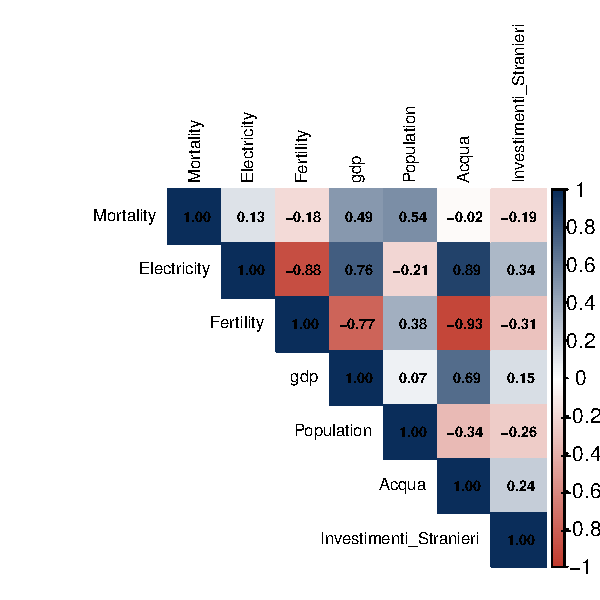
\includegraphics[width=1\linewidth,height=\textheight,keepaspectratio]{presentazione3_files/figure-beamer/plot-corrplot-slide-1.pdf}
\end{column}

\begin{column}{0.5\linewidth}
\small

\textbf{Osservazioni chiave:}

\begin{itemize}
  \item Forte correlazione tra HDI e Mortalità (--0.85).
  \item Elevata collinearità tra PIL, Acqua ed Elettricità.
  \item \textbf{Nota sul VIF:} La mortalità funge da ``proxy'' delle altre variabili, rendendo il VIF matematicamente esplosivo ma economicamente ridondante.
\end{itemize}
\end{column}
\end{columns}
\end{frame}

\begin{frame}{Modelli econometrici: Strategia di stima}
\protect\phantomsection\label{modelli-econometrici-strategia-di-stima}
\begin{itemize}
  \item \textbf{Modello a effetti fissi (PLM)} — controlla per eterogeneità non osservata stabile nel tempo
  \item \textbf{Interazioni variabile $\times$ paese} — slope eterogenei: ogni paese reagisce diversamente ai regressori
  \item \textbf{Errori standard robusti (HC1)} — correggono per eteroschedasticità
  \item Variabili incluse: mortalità, elettricità, fertilità, $\log(\text{GDP})$, accesso all'acqua, FDI
\end{itemize}

\vspace{0.4em}

\textbf{Modello 2} aggiunge dummy di crisi:
\textit{crisi finanziaria 2008--09} e \textit{COVID-19 2020--21}
\end{frame}

\begin{frame}{Modello 1 --- Effetti fissi con interazioni}
\protect\phantomsection\label{modello-1-effetti-fissi-con-interazioni}
Il modello stima l'impatto dei regressori sull'HDI: \[
\text{HDI}_{it} = \alpha_i + \beta_1 \text{Mort}_{it} + \beta_2 \text{Ele}_{it} + \beta_3 \text{Fert}_{it} + \beta_4 \log(\text{GDP})_{it} + \beta_5 \text{Wat}_{it} + \epsilon_{it}
\]

\begin{itemize}
  \item $\alpha_i$: Cattura le caratteristiche specifiche di ogni paese che non variano nel tempo (cultura, posizione geografica, istituzioni storiche).
  \item elimina bias da variabili omesse costanti nel tempo.
  \item Ci permette di vedere come le variazioni \textit{interne} ai paesi influenzano l'HDI.
\end{itemize}
\end{frame}

\begin{frame}{Coefficienti --- Acqua ed Elettricità}
\protect\phantomsection\label{coefficienti-acqua-ed-elettricituxe0}
\begin{tabular}{lrrl}
\toprule
  & Coefficiente & P-value & Significativo\\
\midrule
Acqua & 0.0077 & 0.0000 & ***\\
Nigeria:Acqua & -0.0051 & 0.0008 & ***\\
Senegal:Acqua & -0.0021 & 0.1782 & \\
South Africa:Acqua & 0.0023 & 0.3067 & \\
Electricity & -0.0003 & 0.1767 & \\
\addlinespace
Nigeria:Electricity & 0.0004 & 0.3577 & \\
Senegal:Electricity & 0.0001 & 0.7200 & \\
South Africa:Electricity & 0.0006 & 0.3387 & \\
\bottomrule
\end{tabular}
\end{frame}

\begin{frame}{Coefficienti --- Investimenti Stranieri e log(GDP)}
\protect\phantomsection\label{coefficienti-investimenti-stranieri-e-loggdp}
\resizebox{\textwidth}{!}{
\begin{tabular}{lrrl}
\toprule
  & Coefficiente & P-value & Significativo\\
\midrule
Investimenti\_Stranieri & 0.0013 & 0.0053 & **\\
Nigeria:Investimenti\_Stranieri & 0.0007 & 0.7138 & \\
Senegal:Investimenti\_Stranieri & -0.0004 & 0.6181 & \\
South Africa:Investimenti\_Stranieri & 0.0000 & 0.9745 & \\
log(gdp) & 0.0089 & 0.0330 & *\\
\addlinespace
Nigeria:log(gdp) & 0.0013 & 0.8431 & \\
Senegal:log(gdp) & -0.0044 & 0.5834 & \\
South Africa:log(gdp) & 0.0002 & 0.9837 & \\
\bottomrule
\end{tabular}

}
\end{frame}

\begin{frame}{Coefficienti --- Fertilità e Mortalità}
\protect\phantomsection\label{coefficienti-fertilituxe0-e-mortalituxe0}
\begin{tabular}{lrrl}
\toprule
  & Coefficiente & P-value & Significativo\\
\midrule
Fertility & 0.0272 & 0.0473 & *\\
Nigeria:Fertility & -0.0236 & 0.1342 & \\
Senegal:Fertility & 0.0121 & 0.4129 & \\
South Africa:Fertility & -0.0541 & 0.0077 & **\\
Mortality & 0.0000 & 0.8831 & \\
\addlinespace
Mortality:Nigeria & -0.0003 & 0.3368 & \\
Mortality:Senegal & -0.0006 & 0.0567 & .\\
Mortality:South Africa & -0.0004 & 0.1216 & \\
\bottomrule
\end{tabular}
\end{frame}

\begin{frame}{Modello 2 --- Aggiunta dummy di crisi}
\protect\phantomsection\label{modello-2-aggiunta-dummy-di-crisi}
Abbiamo testato la resilienza dell'HDI agli shock globali:
\[\text{HDI}_{it} = \dots + \beta_1 D_{2008} + \beta_2 D_{2020} + \epsilon_{it}\]

\begin{itemize}
  \item Le dummy di crisi catturano shock macroeconomici esogeni (2008 e COVID-19)
  \item L’obiettivo è verificare se questi eventi hanno avuto un impatto significativo sull’HDI
  \item Le interazioni per paese permettono di valutare eterogeneità nella risposta agli shock
  \item Risultato atteso: possibile maggiore vulnerabilità nei paesi meno sviluppati
\end{itemize}
\end{frame}

\begin{frame}{Coefficienti dummy di crisi}
\protect\phantomsection\label{coefficienti-dummy-di-crisi}
\resizebox{\textwidth}{!}{
\begin{tabular}{lrrl}
\toprule
  & Coefficiente & P-value & Sig.\\
\midrule
crisis\_2008 & 0.0028 & 0.4938 & \\
covid & 0.0056 & 0.3038 & \\
as.factor(country)Nigeria:crisis\_2008 & -0.0060 & 0.2666 & \\
as.factor(country)Senegal:crisis\_2008 & -0.0014 & 0.7936 & \\
as.factor(country)South Africa:crisis\_2008 & 0.0047 & 0.3886 & \\
\addlinespace
as.factor(country)Nigeria:covid & -0.0021 & 0.7705 & \\
as.factor(country)Senegal:covid & -0.0011 & 0.8718 & \\
as.factor(country)South Africa:covid & -0.0048 & 0.4683 & \\
\bottomrule
\end{tabular}

}
\end{frame}

\begin{frame}{Relazione tra reddito e sviluppo umano per paese}
\protect\phantomsection\label{relazione-tra-reddito-e-sviluppo-umano-per-paese}
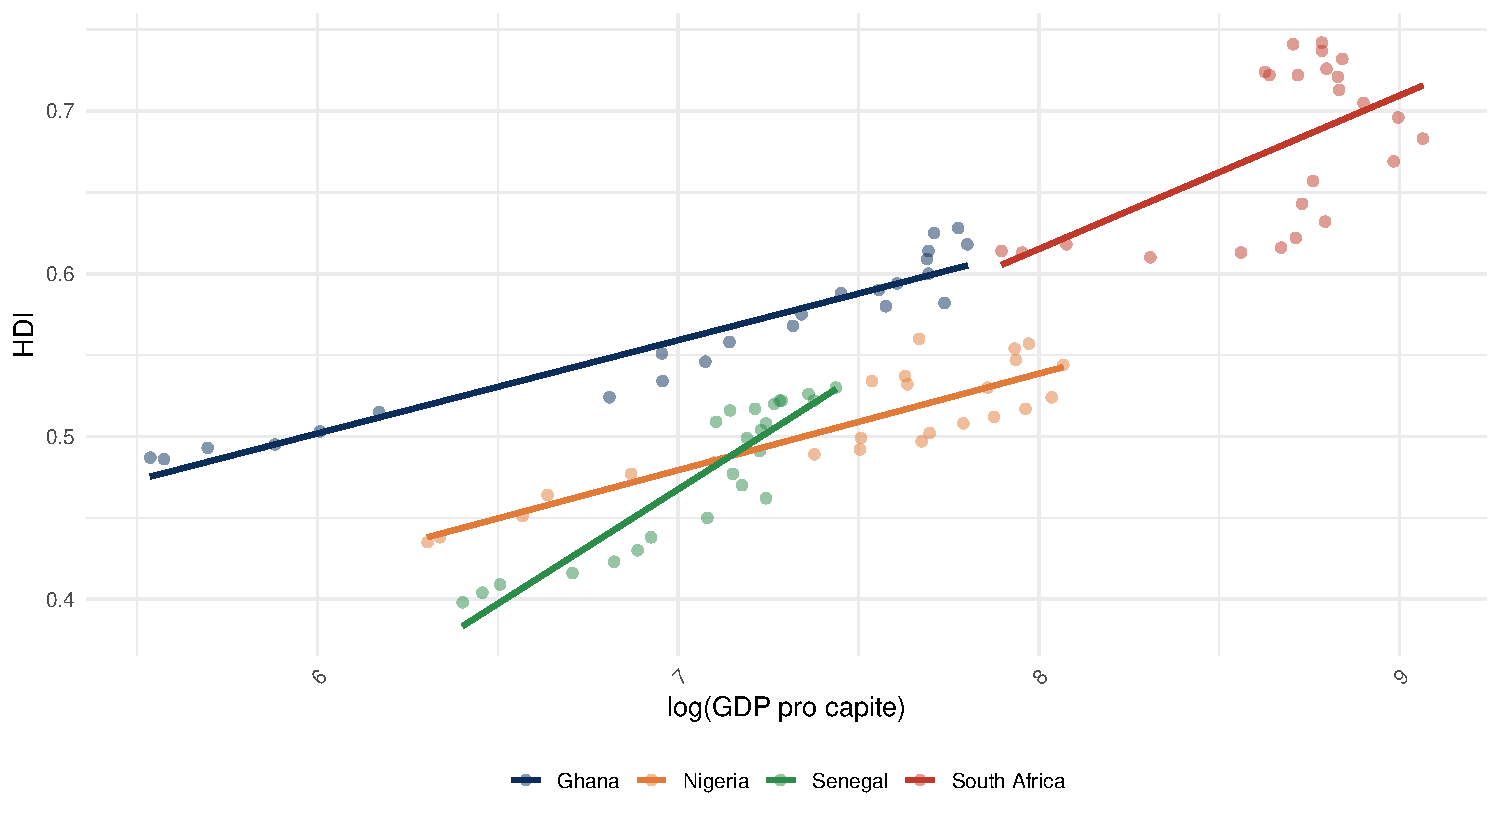
\includegraphics[width=1\linewidth,height=\textheight,keepaspectratio]{presentazione3_files/figure-beamer/plot-gdp-hdi-1.pdf}

\{\footnotesize A parità di crescita del reddito, l'impatto sull'HDI
varia sensibilmente tra paesi.\}
\end{frame}

\begin{frame}{Risultati principali}
\protect\phantomsection\label{risultati-principali}
\begin{itemize}
  \item L'Africa Sub-Sahariana ha migliorato l'HDI dal 1990, ma il \textbf{divario con il livello mondiale rimane ampio}
  \item Il \textbf{Sudafrica} registra l'HDI più alto tra i quattro paesi; la \textbf{Nigeria} il più basso — nonostante il PIL pro capite più elevato della Nigeria rispetto a Ghana e Senegal in alcuni periodi
  \item Il $\log(\text{GDP})$ e la \textbf{fertilità} sono i determinanti con effetti più robusti sull'HDI, ma con pendenze eterogenee per paese
  \item \textbf{Multicollinearità elevata} (VIF $\gg$ 10): mortalità, elettricità e accesso all'acqua sono proxy correlate delle stesse condizioni di sviluppo $\Rightarrow$ modello semplificato preferibile
  \item Le crisi 2008 e COVID-19 hanno avuto impatti differenziati: la Nigeria e il Senegal mostrano maggiore vulnerabilità agli shock esterni
\end{itemize}
\end{frame}

\begin{frame}{Limiti e sviluppi futuri}
\protect\phantomsection\label{limiti-e-sviluppi-futuri}
\begin{itemize}
  \item Campione ridotto (4 paesi, 34 anni): potere statistico limitato per i test di diagnostica
  \item Possibile \textbf{autocorrelazione seriale} nei residui — stimatori GMM come alternativa
  \item Estendere l'analisi ad altri paesi dell'Africa Sub-Sahariana per una maggiore generalizzabilità
  \item Includere variabili istituzionali (governance, rule of law) come determinanti non economici dell'HDI
\end{itemize}

\vspace{0.5em}
\begin{center}
\textit{Grazie per l'attenzione}
\end{center}
\end{frame}




\end{document}
